\documentclass{beamer}

% --- Theme Selection ---
\usetheme{Berlin}

% --- Packages ---
\usepackage{graphicx}
\usepackage{booktabs}
\usepackage{array}
\usepackage{multirow}
\usepackage{makecell}
\usepackage{pifont}
\usepackage{tikz}
\usetikzlibrary{arrows.meta, positioning}

% --- Graphics ---
\graphicspath{{figures/}}

% --- Small presentation helpers ---
\setbeamertemplate{navigation symbols}{}
\newcommand{\smallgap}{\vspace{0.15cm}}
\newcommand{\source}[1]{\vfill{\tiny\color{gray}#1}}
\newcommand{\cmark}{\textcolor{green!55!black}{\ding{51}}}
\newcommand{\xmark}{\textcolor{red!70!black}{\ding{55}}}
\newcommand{\pilltag}[1]{\colorbox{structure!12}{\scriptsize\strut\,#1\,}}

% --- Title Page Information ---
\title{LymphNode}
\subtitle{A Plug-and-Play Access Control Method for Deep Neural Networks}
\author{Hanyu Pei \and Shang Liu \and Zeyan Liu}
\institute{University of Louisville}
\date{DSN 2026}

\begin{document}

% --- Title Slide ---
\frame{\titlepage}

% --- Table of Contents ---
\begin{frame}
\frametitle{Outline}
\tableofcontents
\end{frame}

% --- Section 1: Motivation ---
\section{Background}

\begin{frame}{AI Is Everywhere}
    \begin{columns}[T,totalwidth=\textwidth]
        \begin{column}{0.55\textwidth}
            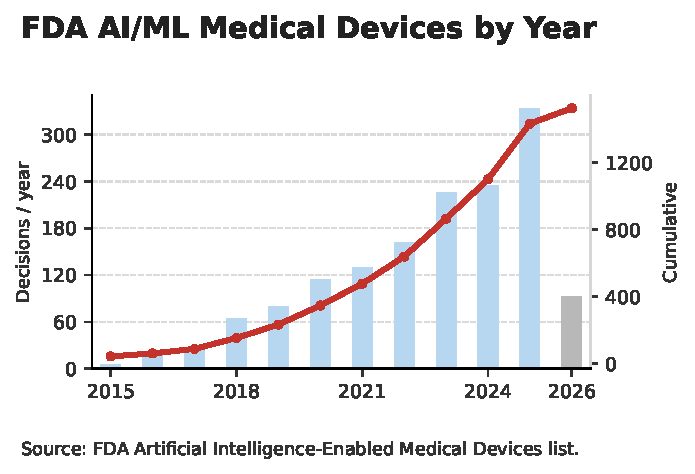
\includegraphics[width=\textwidth]{fda_aiml_devices_by_year.pdf}
            \vspace{-0.1cm}
            {\scriptsize Concrete example: FDA-cleared \textbf{AI/ML medical devices} per year --- growing fast.}
        \end{column}
        \begin{column}{0.43\textwidth}
            \small
            DNNs now power everyday products:
            \begin{itemize}
                \setlength\itemsep{0.14cm}
                \item Healthcare \& diagnosis
                \item Finance \& fraud detection
                \item Autonomous driving
                \item Phones \& assistants
            \end{itemize}
            \smallgap
            \begin{block}{Why it matters}
                \small Each model $=$ months of compute $+$ private data $\Rightarrow$ \textbf{valuable IP worth stealing}.
            \end{block}
        \end{column}
    \end{columns}
\end{frame}

\begin{frame}{DNNs at the Edge Are Exposed}
    \centering
    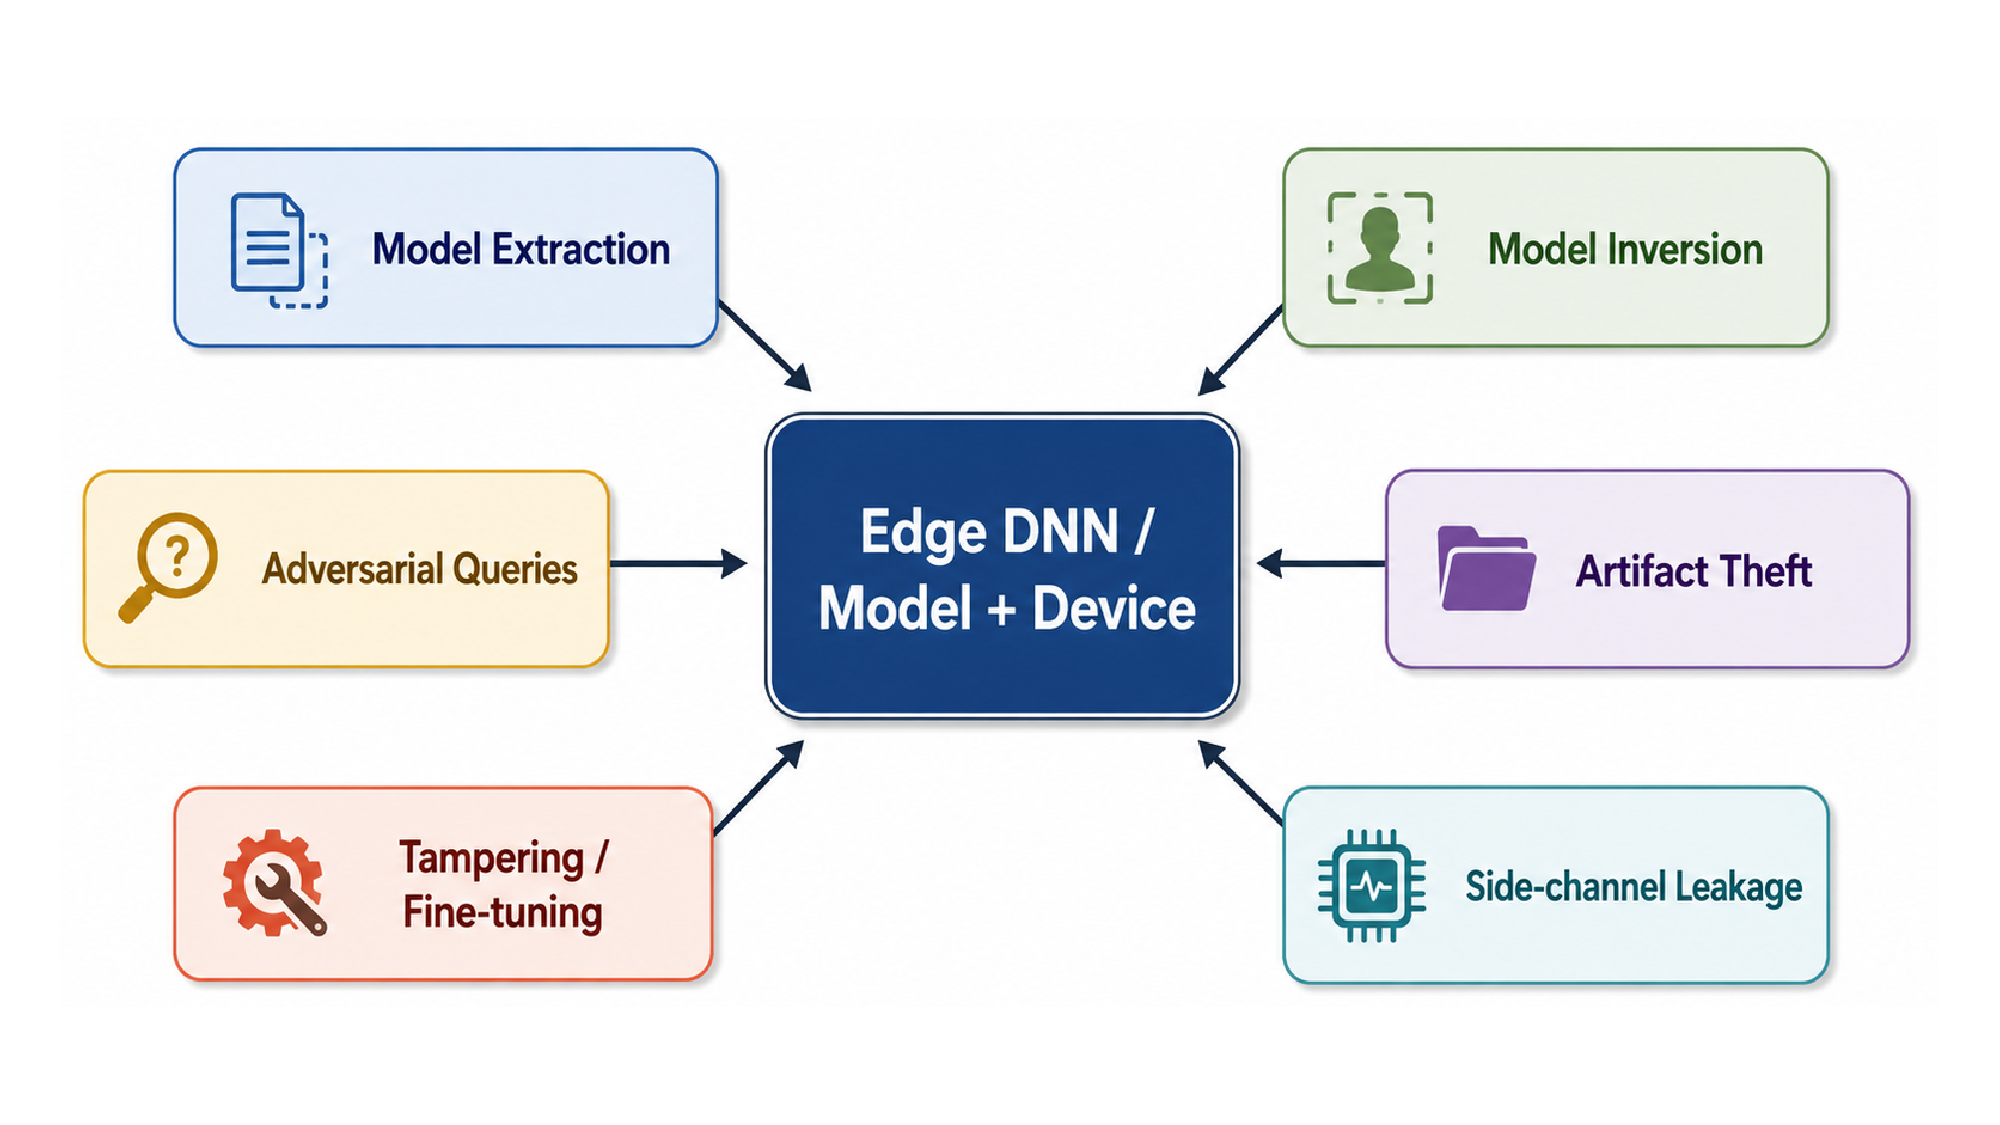
\includegraphics[width=0.95\textwidth,keepaspectratio]{edge_dnn_threats_no_title.pdf}

\end{frame}

\begin{frame}{Attack Surface and Defense Surface}
    \begin{columns}[T,totalwidth=\textwidth]
        \begin{column}{0.48\textwidth}
            \textbf{Attack surface}
            \small
            \begin{itemize}
                \setlength\itemsep{0.22cm}
                \item Query-response pairs expose model behavior.
                \item Confidence scores can leak private training information.
                \item Deployed artifacts invite removal or fine-tuning attempts.
            \end{itemize}
        \end{column}
        \begin{column}{0.48\textwidth}
            \textbf{Defense surface}
            \small
            \begin{itemize}
                \setlength\itemsep{0.22cm}
                \item Prove ownership after theft.
                \item Perturb outputs at the service interface.
                \item Lock weights or structure during training.
                \item Enforce access control inside the deployed model.
            \end{itemize}
        \end{column}
    \end{columns}
    \vspace{0.2cm}

\end{frame}

% --- Section 2: Related Work ---
\section{Related Work}

\begin{frame}{Existing Defenses at a Glance --- and the Gap}
    \footnotesize
    \begin{center}
    \setlength{\tabcolsep}{6pt}\renewcommand{\arraystretch}{1.35}
    \begin{tabular}{lccccc}
        \toprule
        \textbf{Defense family} & \makecell{\textbf{Prevent}\\\textbf{use}} & \makecell{\textbf{No orig.}\\\textbf{data}} & \makecell{\textbf{No}\\\textbf{retrain}} & \makecell{\textbf{Edge-}\\\textbf{ready}} & \textbf{Overhead} \\
        \midrule
        Watermark / fingerprint & \xmark & \xmark & \xmark & \cmark & Low \\
        Output poisoning        & \cmark & \cmark & \cmark & \xmark & Per-query \\
        Crypto / hardware lock  & \cmark & \cmark & \cmark & \xmark & High \\
        Train-time lock         & \cmark & \xmark & \xmark & \cmark & Low \\
        \midrule
        \textbf{LymphNode}      & \cmark & \cmark & \cmark & \cmark & \textbf{Negligible} \\
        \bottomrule
    \end{tabular}
    \end{center}
    \smallgap
    \scriptsize \textbf{Representative works} --- watermark/fingerprint: Uchida, Adi, DeepSigns, IPGuard; output poisoning: PP, CIP, AMAO; crypto/HW: Deep-Lock, NN-Lock, TEE, HE; train-time lock: AdvParams, SSAT, ModelLock, IDEA.

\end{frame}


% --- Section 3: LymphNode Design ---
\section{LymphNode Design}

\begin{frame}{Our Goal: A Lightweight Security Plugin}

    \begin{itemize}
        \setlength\itemsep{0.18cm}
        \item \textbf{Active} --- neutralize unauthorized inputs by default, not just prove ownership after theft.
        \item \textbf{Lightweight} --- constant, near-zero inference overhead; runs at the edge, no server.
        \item \textbf{Plug-and-play} --- post-hoc add-on, no retraining or model surgery.
        \item \textbf{Data-light} --- set up with few data, even a public surrogate; no original training set.
    \end{itemize}
    \vspace{0.35cm}
    \begin{center}
        \pilltag{Active} \pilltag{Lightweight} \pilltag{Plug-and-play} \pilltag{Data-light}
    \end{center}
\end{frame}

\begin{frame}{Threat Model: Edge Deployment, Oracle-Only Adversary}
    \begin{columns}[T,totalwidth=\textwidth]
        \begin{column}{0.49\textwidth}
            \begin{block}{Three honest parties}
                \begin{minipage}[t][2.7cm][t]{\linewidth}
                \footnotesize
                \textbf{Model owner} --- trains the model, optimizes the GSUAP plugin, issues keys.\\[3pt]
                \textbf{Edge operator} --- deploys inside a trusted runtime; distributes keys.\\[3pt]
                \textbf{Authorized user} --- submits inputs carrying the credential.
                \end{minipage}
            \end{block}
        \end{column}
        \begin{column}{0.49\textwidth}
            \begin{alertblock}{Gray-box adversary}
                \begin{minipage}[t][2.7cm][t]{\linewidth}
                \footnotesize
                \textbf{Knows:} architecture $+$ defense mechanism.\\[3pt]
                \textbf{Cannot access:} secret key $\mathbf{k}$, intermediate feature maps, gradients / backward pass.\\[3pt]
                \textbf{Only weapon:} unlimited oracle queries (incl.\ adaptive).
                \end{minipage}
            \end{alertblock}
        \end{column}
    \end{columns}
    \vspace{0.2cm}
    \centering\footnotesize At the edge there is no server to filter queries --- protection must live \emph{inside} the forward pass.
\end{frame}

\begin{frame}{System Overview}
    \centering
    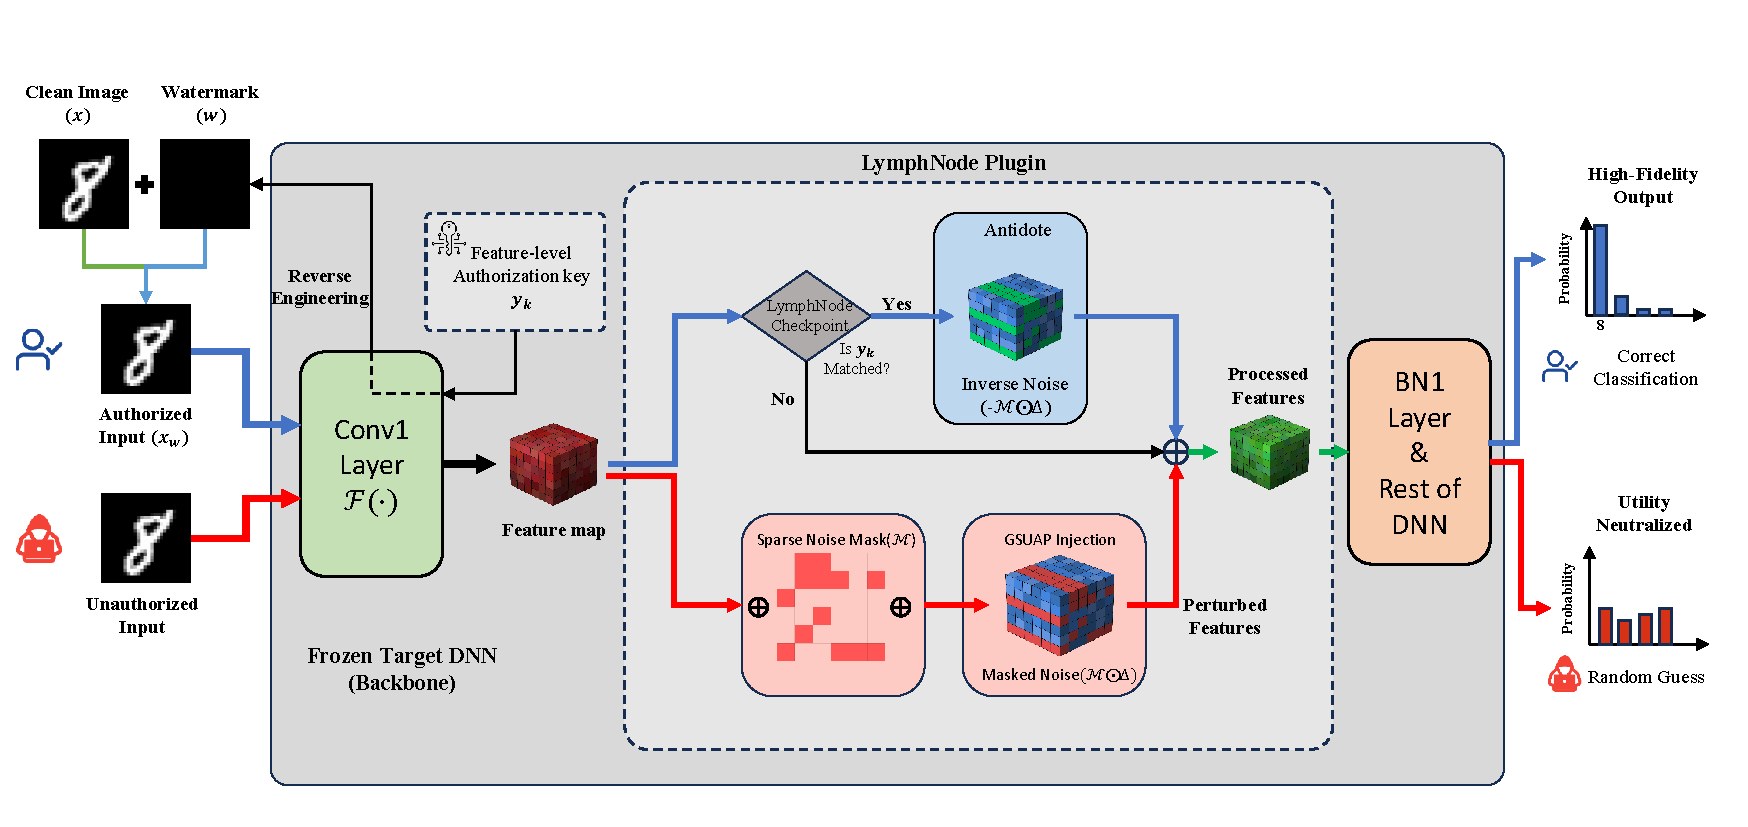
\includegraphics[width=\textwidth,height=\textheight,keepaspectratio]{framework.pdf}

\end{frame}

\begin{frame}{Component 1 --- Feature-Domain Credential}
    \centering
    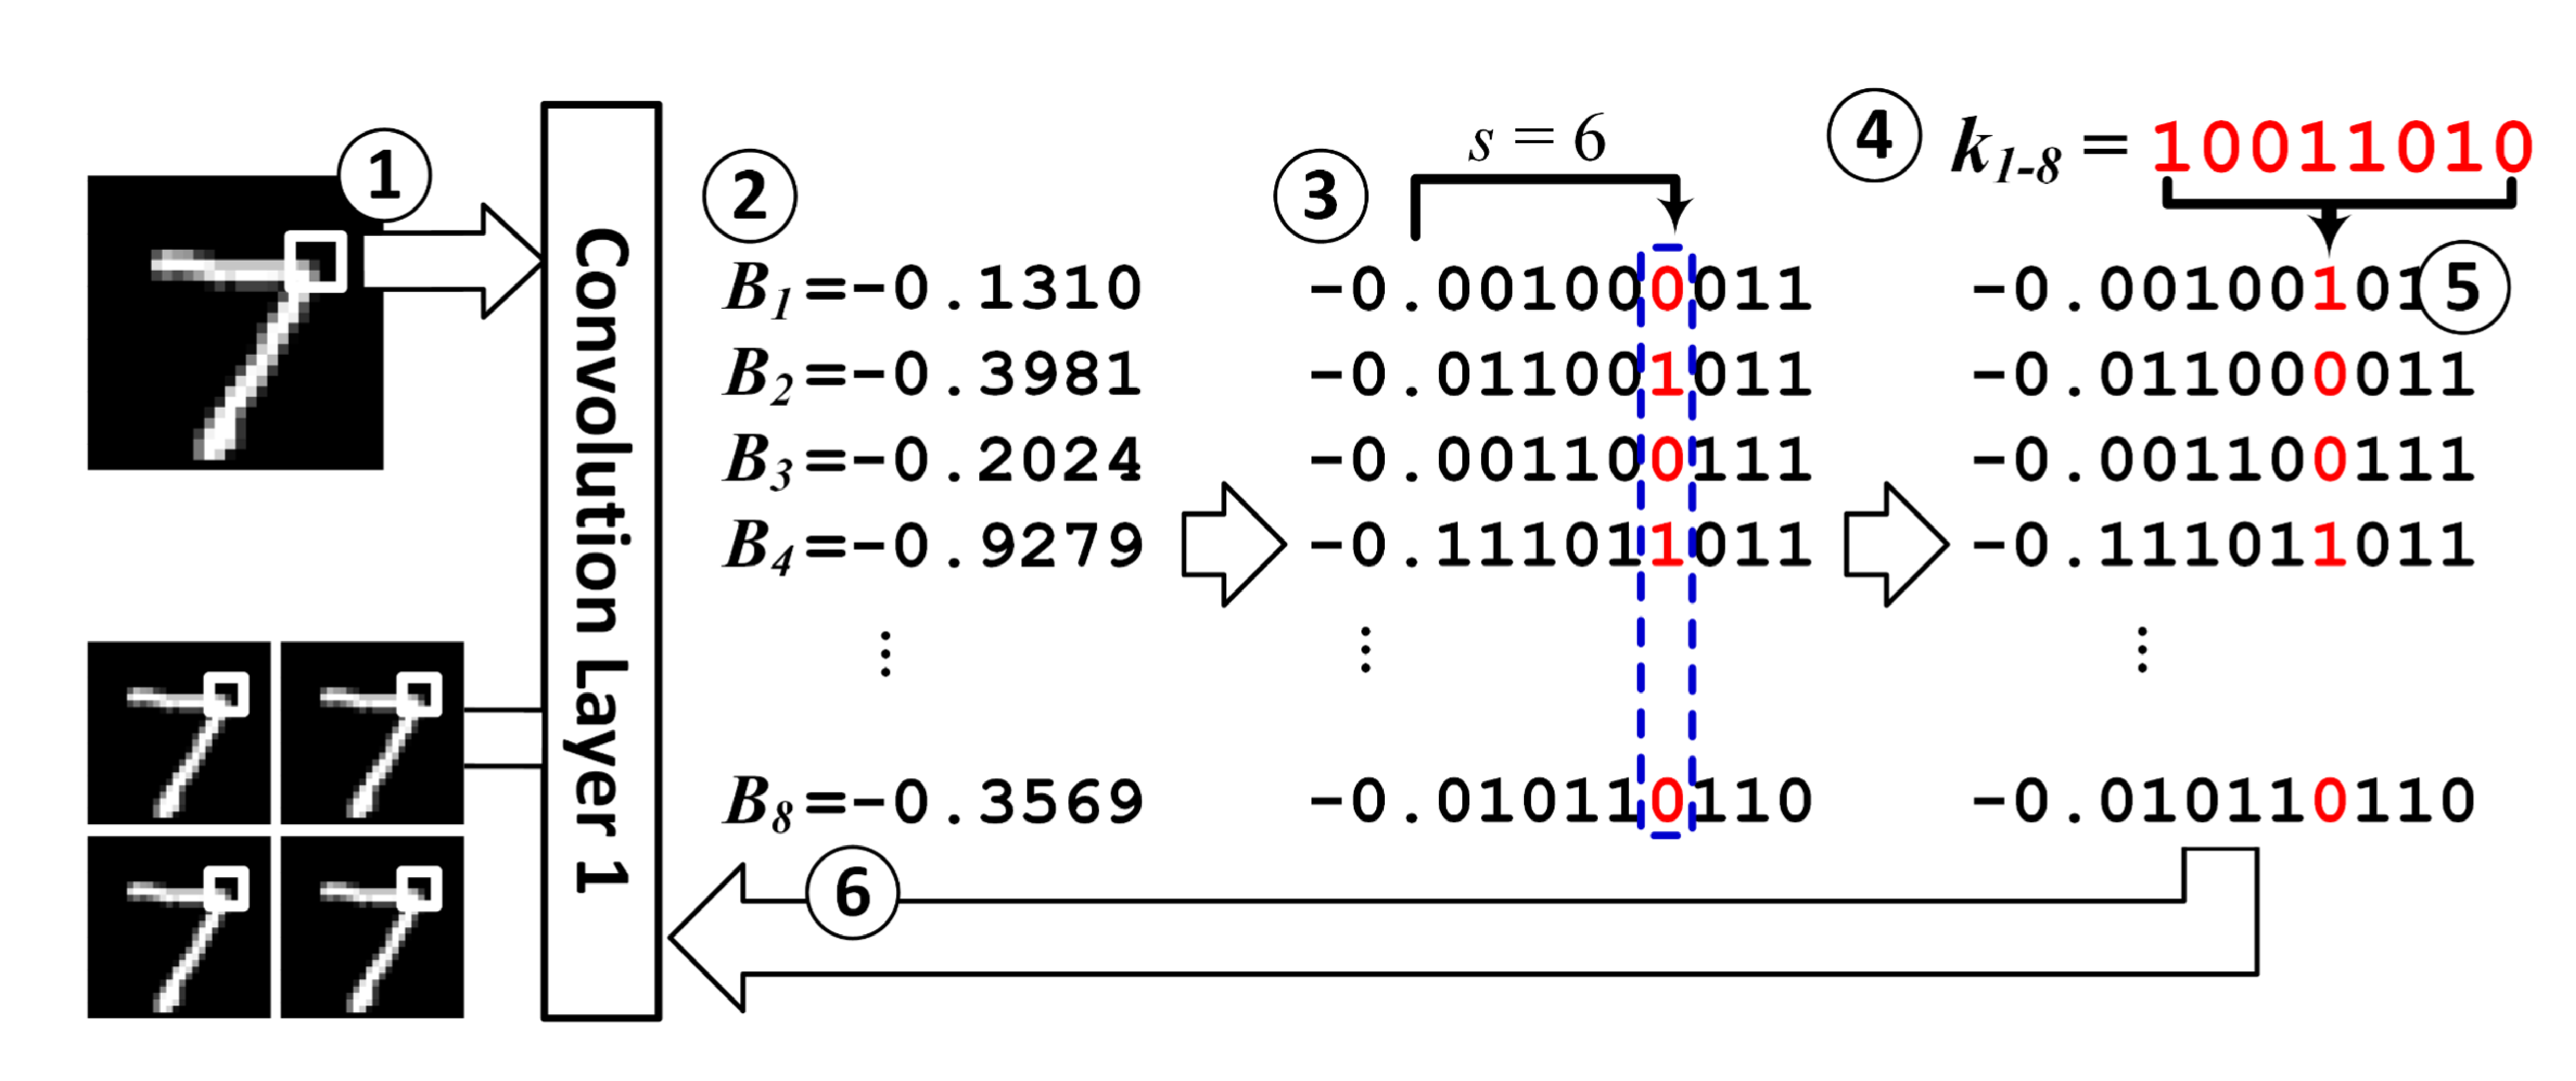
\includegraphics[width=\textwidth,height=0.5\textheight,keepaspectratio]{LSB_key.pdf}
    \vspace{0.15cm}

    \scriptsize
    \begin{columns}[T,totalwidth=\textwidth]
        \begin{column}{0.5\textwidth}
            \ding{192}~~Input $x$ passes through conv layer 1.\\[3pt]
            \ding{193}~~Read $N$ carrier features $B_1,\dots,B_N$.\\[3pt]
            \ding{194}~~Inspect each at depth $s$.
        \end{column}
        \begin{column}{0.5\textwidth}
            \ding{195}~~Construct secret key $\mathbf{k}=1001\,1010\dots$\\[3pt]
            \ding{196}~~Flip bits at $s$ so features encode $\mathbf{k}$.\\[3pt]
            \ding{197}~~Invert to pixels: $x{+}\mathbf{w}$ carry the key.
        \end{column}
    \end{columns}
    \vspace{0.15cm}
    \centering\footnotesize Modifying only the $s$-th bit keeps the change at the level of quantization noise invisible in pixels, yet an exact, discrete match on verification.
\end{frame}

\begin{frame}{Component 1 --- Generation \& Collision}
    \begin{itemize}\small
        \item \textbf{Key:} secret $\mathbf{k}\in\{0,1\}^{N}$, $N{=}32$ bits over $v{=}4$ kernels; each bit read at depth $s{=}6$: $b=\lfloor |y|\cdot 2^{s}\rfloor \bmod 2$.
        \item \textbf{Generation:} find a tiny pixel perturbation $\mathbf{w}$ by random search so $\mathbf{x}{+}\mathbf{w}$'s features match $\mathbf{k}$ --- complexity $O(h\cdot 2^{v})$, \textbf{1000 credentials in $<2$\,s}.
        \item \textbf{Verification:} re-extract the 32 bits and compare --- a cheap discrete check, no optimization.
    \end{itemize}
    \vspace{0.2cm}
    \begin{block}{Collision analysis}
        \small Probability an unauthorized input matches all $N{=}32$ bits: $P_c = 2^{-N}\approx 2.3\times10^{-10}$. \textbf{No collision observed across all experiments.}
    \end{block}
\end{frame}

\begin{frame}{Component 2 --- GSUAP Neutralization}
    \textbf{Idea:} inject \textbf{GSUAP} --- a \emph{Generalized Sparse Universal Adversarial Perturbation}, i.e.\ a static \textbf{adversarial noise} --- into the features to destroy utility for unauthorized inputs while touching as few channels as possible.
    \smallgap
    \begin{enumerate}\small
        \item \textbf{Rank channels} by gradient sensitivity on a tiny calibration set:
        $\;\text{Score}_j=\mathbb{E}\big[\,\|\partial \mathcal{L}_{CE}/\partial W_j\|_2\,\big]$.
        \item \textbf{Sparse mask} $\mathcal{M}$: keep the top-$k$ ($k=\lfloor rM\rfloor$) decision-critical channels.
        \item \textbf{Optimize one universal $\Delta$} by projected gradient \emph{ascent} ($\|\Delta\|_\infty\le\epsilon$) to wreck clean accuracy:
        \[ \widetilde{F}(x) = F(x) + \mathcal{M} \odot \Delta \]
        \item \textbf{Default-on:} unauthorized $\to$ add $\Delta$; authorized $\to$ inverse $\Delta$ (antidote) cancels it.
    \end{enumerate}
    \vspace{0.05cm}

\end{frame}

\begin{frame}{Inference Logic}
    \begin{center}
    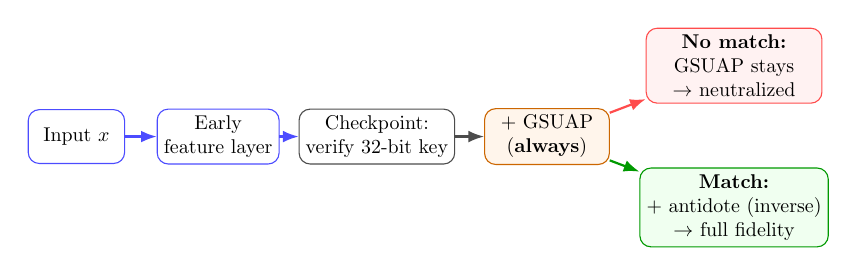
\begin{tikzpicture}[
        scale=0.72, transform shape,
        box/.style={draw, rounded corners, align=center, minimum height=0.95cm},
        arr/.style={-{Latex[length=2mm]}, thick}
    ]
        \node[box, draw=blue!70, minimum width=1.7cm] (input) at (0,0) {Input $x$};
        \node[box, draw=blue!70, minimum width=2.0cm] (feat) at (2.5,0) {Early\\feature layer};
        \node[box, draw=black!70, minimum width=2.4cm] (check) at (5.3,0) {Checkpoint:\\verify 32-bit key};
        \node[box, draw=orange!80!black, fill=orange!8, minimum width=2.2cm] (gsuap) at (8.3,0) {$+$ GSUAP\\(\textbf{always})};
        \node[box, draw=red!70, fill=red!5, minimum width=3.1cm] (bad) at (11.6,1.25) {\textbf{No match:}\\GSUAP stays\\$\to$ neutralized};
        \node[box, draw=green!60!black, fill=green!6, minimum width=3.1cm] (good) at (11.6,-1.25) {\textbf{Match:}\\$+$ antidote (inverse)\\$\to$ full fidelity};
        \draw[arr, blue!70] (input) -- (feat);
        \draw[arr, blue!70] (feat) -- (check);
        \draw[arr, black!70] (check) -- (gsuap);
        \draw[arr, red!70] (gsuap) -- (bad);
        \draw[arr, green!60!black] (gsuap) -- (good);
    \end{tikzpicture}
    \end{center}
    \vspace{0.3cm}
    \centering\footnotesize  GSUAP is always injected; only a verified credential also adds the antidote (inverse GSUAP) that cancels it.
\end{frame}

% --- Section 4: Experimental Results ---
\section{Experimental Results}

\begin{frame}{Experimental Setup}
    \begin{itemize}\small
        \item \textbf{Datasets:} CIFAR-10, MNIST, SVHN ($+$ CIFAR-100/STL-10 transfer, CelebA inversion).
        \item \textbf{Architectures:} ResNet-18/50, ViT-Tiny/Small, DenseNet, AlexNet.
        \item \textbf{Baselines:} Gaussian, SUAP; PP, CIP (extraction/inversion); BadNets, Blended, Passport (robustness).
    \end{itemize}
    %每个实验各自说，这里有问题
    \vspace{0.25cm}
    \centering\footnotesize Five questions: \textbf{Does it lock out? At what cost? Against real attacks? With how little data? How robust?}
\end{frame}

\begin{frame}{Result 1 --- Unauthorized Queries Are Locked Out}
    \scriptsize
    \begin{center}
    \setlength{\tabcolsep}{5pt}
    \renewcommand{\arraystretch}{1.2}
    \resizebox{\textwidth}{!}{%
    \begin{tabular}{ll | rrrr | rrrr}
        \toprule
        \multirow{2}{*}{\textbf{Model}} & \multirow{2}{*}{\textbf{Ratio}}
        & \multicolumn{4}{c|}{\textbf{CIFAR-10}}
        & \multicolumn{4}{c}{\textbf{MNIST}} \\
        \cmidrule(lr){3-6} \cmidrule(lr){7-10}
        & & Gauss & SUAP & GSUAP & VIP & Gauss & SUAP & GSUAP & VIP \\
        \midrule
        \multirow{5}{*}{ResNet-18}
          & 20  & 93.6 & 93.2 & \textbf{88.6} & 94.5 & 49.0 & 10.2 & \textbf{10.2} & 99.6 \\
          & 40  & 87.4 & 81.4 & \textbf{36.4} & 94.5 & 31.3 & 11.3 & \textbf{11.3} & 99.6 \\
          & 60  & 85.4 & 72.0 & \textbf{13.6} & 94.5 & 29.4 & 9.3  & \textbf{9.3}  & 99.6 \\
          & 80  & 80.2 & 67.0 & \textbf{11.0} & 94.5 & 24.7 & 10.6 & \textbf{10.2} & 99.6 \\
          & 100 & 73.6 & 48.4 & \textbf{10.6} & 94.5 & 22.6 & 10.2 & \textbf{10.2} & 99.6 \\
        \midrule
        \multirow{5}{*}{ViT-Tiny}
          & 20  & 71.6 & 49.0 & \textbf{27.8} & 91.8 & 46.3 & 11.2 & \textbf{10.4} & 99.3 \\
          & 40  & 51.0 & 16.6 & \textbf{11.6} & 91.8 & 32.4 & 10.9 & \textbf{10.0} & 99.3 \\
          & 60  & 39.8 & 13.6 & \textbf{11.8} & 91.8 & 23.8 & 9.4  & \textbf{8.9}  & 99.3 \\
          & 80  & 34.8 & 11.8 & \textbf{10.6} & 91.8 & 21.2 & 9.9  & \textbf{8.4}  & 99.3 \\
          & 100 & 29.8 & 11.2 & \textbf{10.6} & 91.8 & 19.0 & 9.8  & \textbf{8.4}  & 99.3 \\
        \bottomrule
    \end{tabular}}
    \end{center}

    \vspace{0.12cm}
    \footnotesize
    \textbf{Ratio}: \% of channels with GSUAP injection. Gauss / SUAP / GSUAP = unauthorized accuracy ($\downarrow$); VIP = authorized accuracy ($\uparrow$).

    \vspace{0.08cm}
    \begin{itemize}\footnotesize
        \item \textbf{GSUAP $\to$ near-random}, monotone in ratio; \textbf{VIP unchanged}.
        \item Hard case (ResNet-18 / CIFAR-10): Gauss 85.4, SUAP 72.0, \textbf{GSUAP 13.6}.
    \end{itemize}
\end{frame}

\begin{frame}{Result 2 ---High channel efficiency}
    \centering
    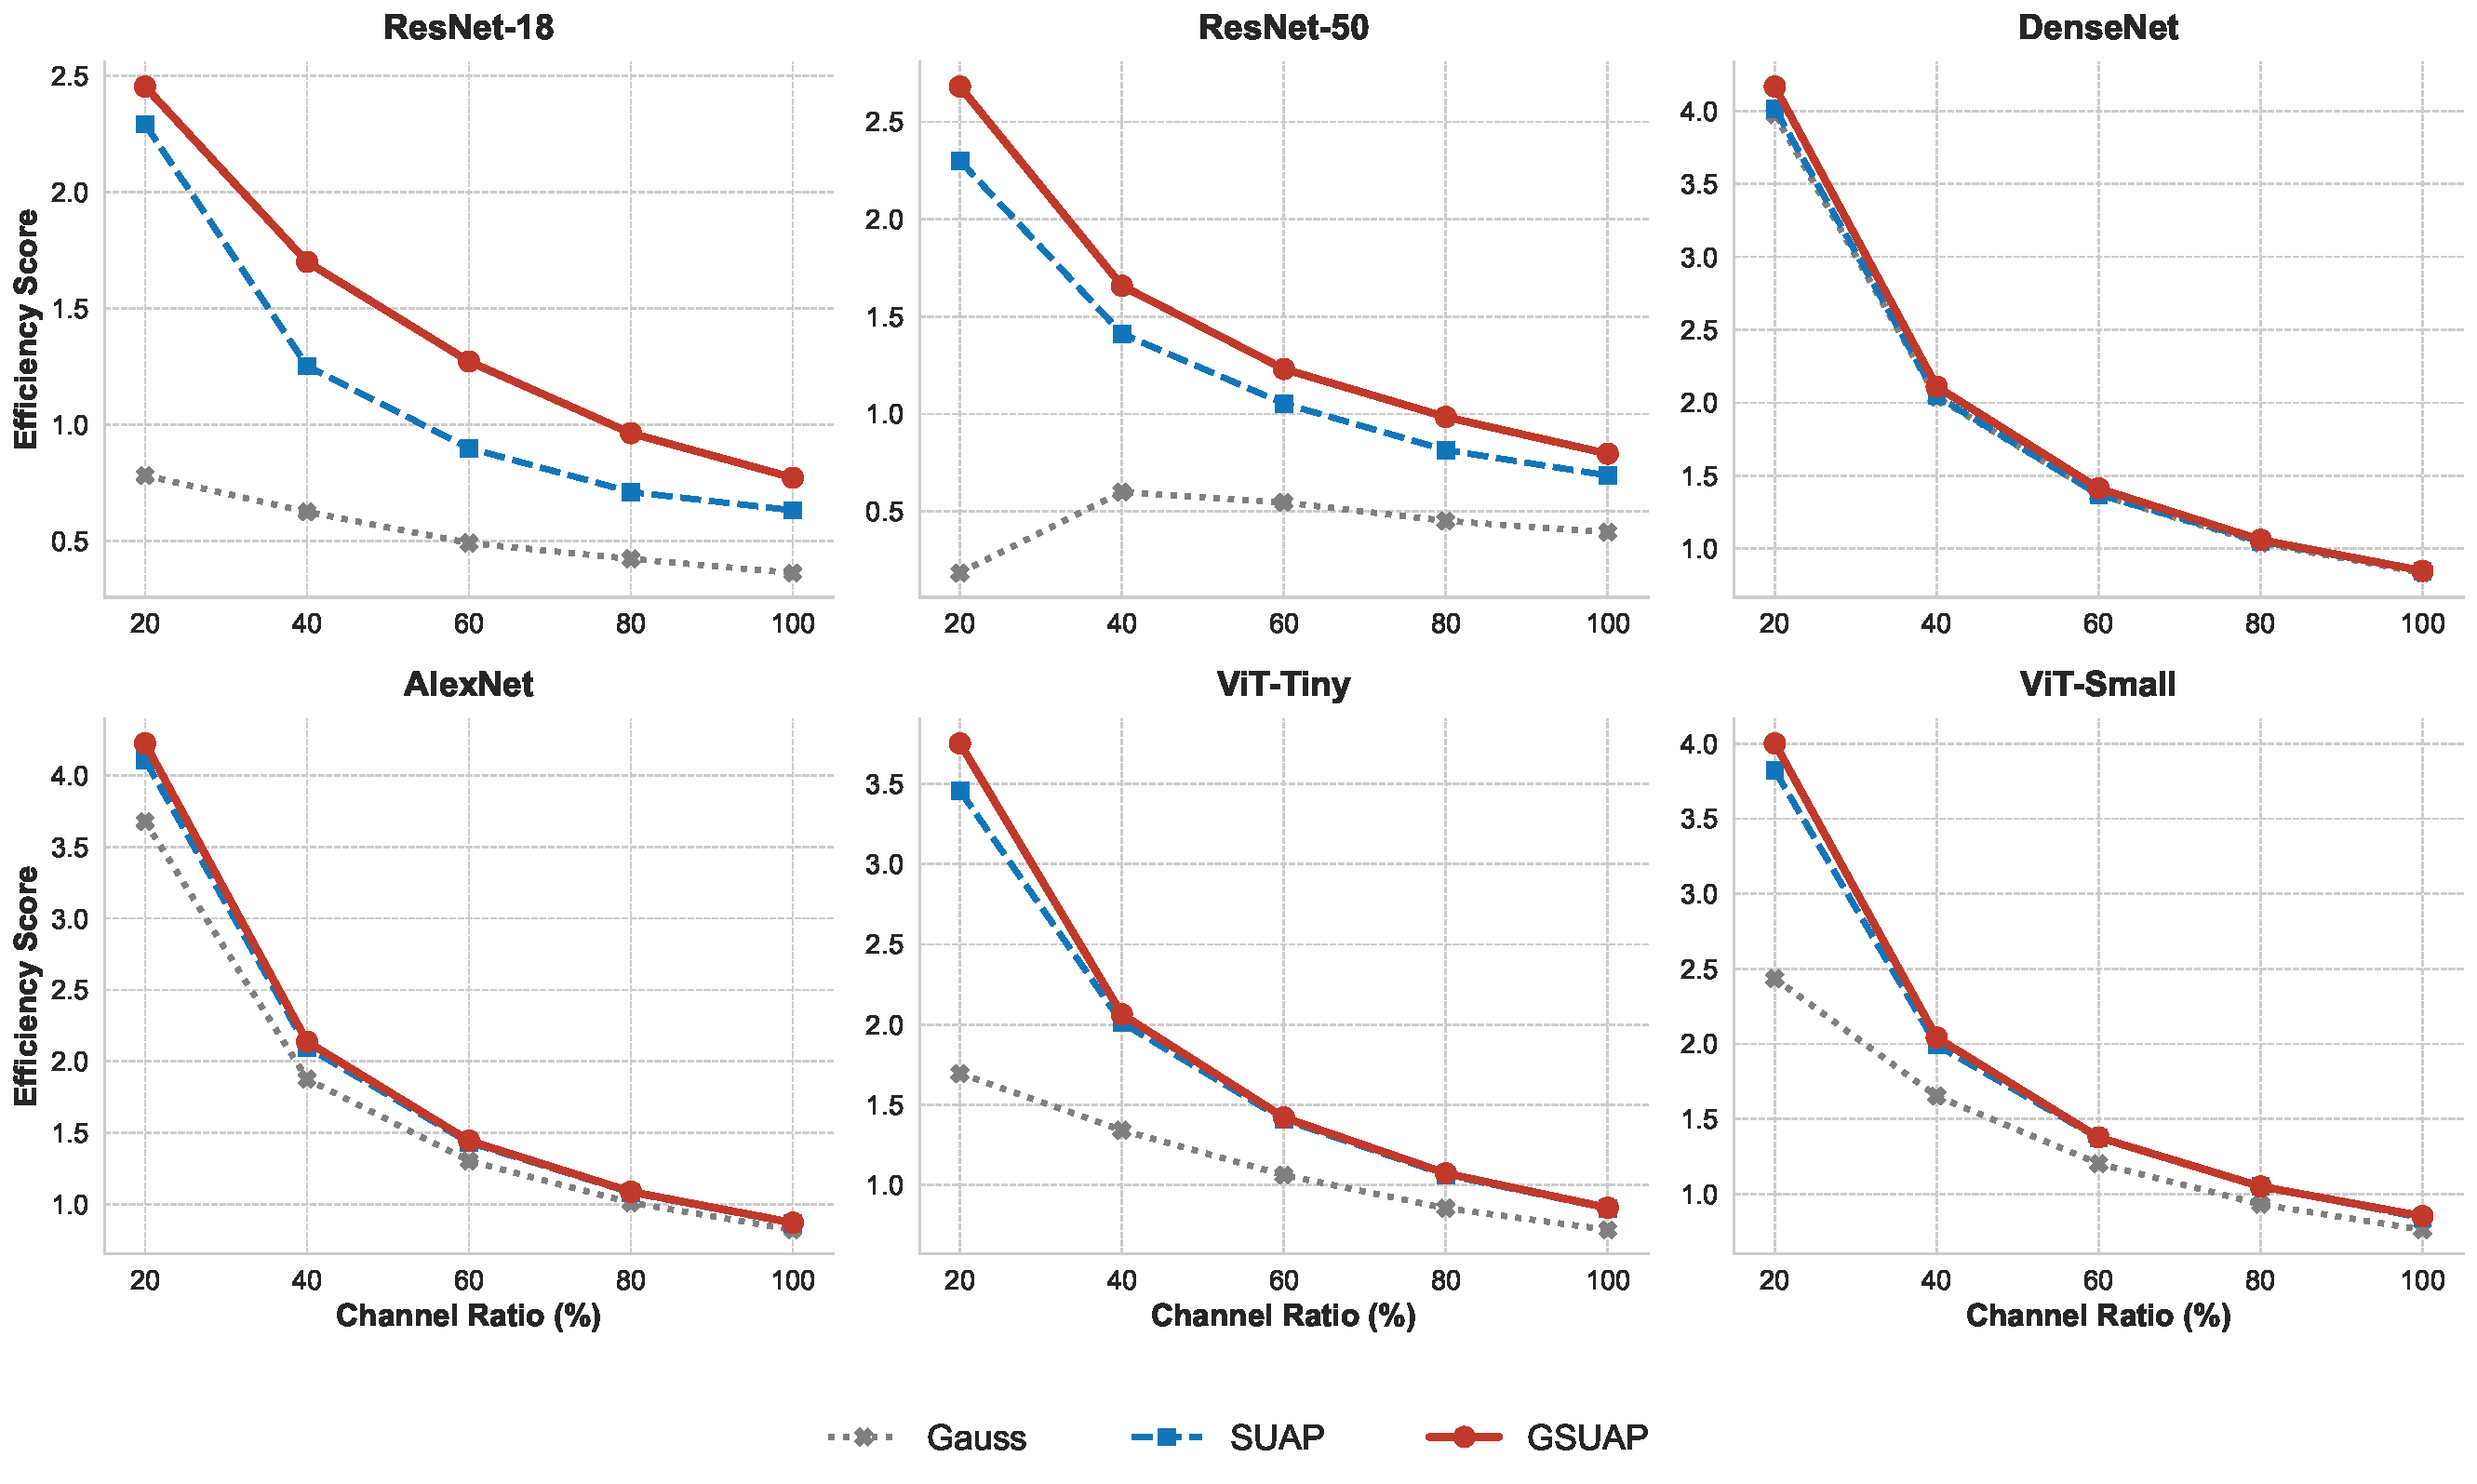
\includegraphics[width=\textwidth,height=0.66\textheight,keepaspectratio]{efficiency_comparison.pdf}
    \vspace{0.1cm}
    \begin{center}\footnotesize
        $E=(\mathcal{A}_{\text{auth}}-\mathcal{A}_{\text{unauth}})/\rho$ --- protection per modified channel. \textbf{GSUAP $\approx$2.5 @20\%} vs Gaussian $<$0.8; gap widens on robust ResNets / ViTs.
    \end{center}
\end{frame}

\begin{frame}{Result 3 --- Constant, Near-Zero Overhead}
    \small
    \begin{center}
    \setlength{\tabcolsep}{5pt}\renewcommand{\arraystretch}{1.3}
    \begin{tabular}{l | ccc | ccc}
        \toprule
        \multirow{2}{*}{\textbf{Metric}} & \multicolumn{3}{c|}{\textbf{ResNet-18}} & \multicolumn{3}{c}{\textbf{ViT-Tiny}} \\
        \cmidrule(lr){2-4}\cmidrule(lr){5-7}
         & Clean & Prot. & \textbf{Cost} & Clean & Prot. & \textbf{Cost} \\
        \midrule
        Params (M)      & 11.17 & 11.17 & $+0.0\%$       & 1.80  & 1.80  & $+0.0\%$ \\
        FLOPs (G)       & 0.558 & 0.558 & ${\approx}0$   & 0.118 & 0.118 & ${\approx}0$ \\
        Latency (ms)    & 1.70  & 2.74  & \textbf{+1.0}  & 1.54  & 2.60  & \textbf{+1.1} \\
        Throughput (/s) & 6893  & 5875  & $-14.8\%$      & 17175 & 16023 & $-6.7\%$ \\
        Memory (MB)     & 93.2  & 109.2 & $+17.2\%$      & 33.7  & 35.2  & $+4.5\%$ \\
        \bottomrule
    \end{tabular}
    \end{center}
    \vspace{0.3cm}
    \centering\footnotesize Params / FLOPs \textbf{unchanged} $\cdot$ latency \textbf{+${\sim}1$\,ms constant} $\cdot$ no per-query cost $\Rightarrow$ fits 30\,FPS (33\,ms).
\end{frame}

\begin{frame}{Result 4 --- Holds Against Real Attack Pipelines}
    \scriptsize
    \begin{center}
    \textbf{Model extraction --- KnockoffNets surrogate accuracy} (\%, $\downarrow$)\\[2pt]
    \setlength{\tabcolsep}{8pt}\renewcommand{\arraystretch}{1.1}
    \begin{tabular}{lcccc}
        \toprule
        \textbf{Query budget} & No def. & PP & CIP & \textbf{LymphNode} \\
        \midrule
        1{,}000  & 42.88 & 25.26 & 28.44 & \textbf{13.71} \\
        5{,}000  & 56.25 & 32.68 & 35.17 & \textbf{14.76} \\
        10{,}000 & 66.16 & 38.24 & 42.81 & \textbf{14.68} \\
        50{,}000 & 85.24 & 45.66 & 48.25 & \textbf{15.28} \\
        \bottomrule
    \end{tabular}
    \end{center}

    \vspace{0.18cm}
    \begin{center}
    \textbf{Model inversion --- GMI (black-box), CelebA, 50 identities}\\[2pt]
    \setlength{\tabcolsep}{8pt}\renewcommand{\arraystretch}{1.1}
    \begin{tabular}{lcccc}
        \toprule
        \textbf{Defense} & Acc-1\,$\downarrow$ & Acc-5\,$\downarrow$ & KNN Dist\,$\uparrow$ & Latency \\
        \midrule
        None (clean) & 82.71 & 91.32      & 5.57   & 0.082\,ms \\
        CIP          & 44.30 & 48.23      & 6.45   & 0.110\,ms \\
        PP           & 3.02  & 8.77       & 7.71   & 0.308\,ms \\
        \textbf{LymphNode} & 4.17 & 11.22 & 7.51   & \textbf{0.088\,ms} \\
        \bottomrule
    \end{tabular}
    \end{center}
\end{frame}

\begin{frame}{Result 5 --- Data Efficiency}
    \centering
    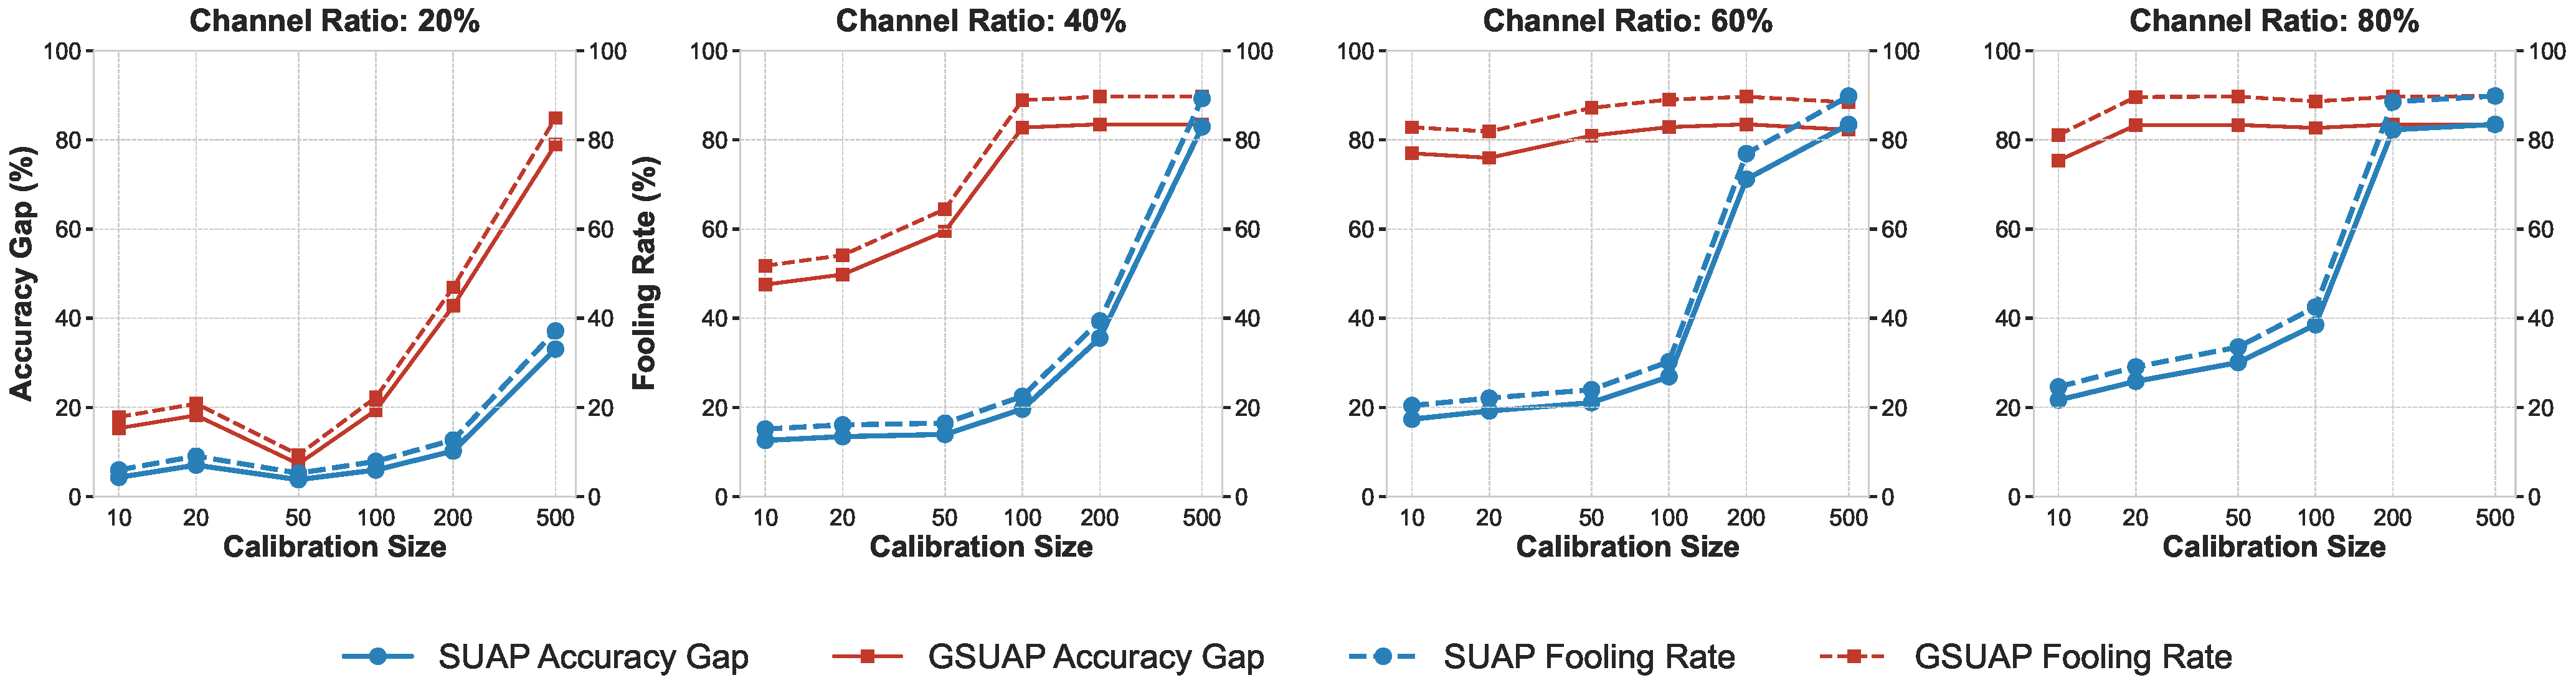
\includegraphics[width=\textwidth,height=0.6\textheight,keepaspectratio]{exp3_visualization.pdf}

    \vspace{0.12cm}
    \begin{itemize}\footnotesize
        \item Calibration size $10\to500$ ($\le 1\%$ of data).
        \item $\ge 40\%$ ratio: robust lockout from \textbf{50--100 samples}; 60--80\% saturates instantly --- \textbf{$\gg$ SUAP}.
    \end{itemize}
    \vspace{0.05cm}
    {\scriptsize Accuracy Gap $=\mathcal{A}_{\text{auth}}-\mathcal{A}_{\text{unauth}}$; \textbf{Fooling Rate (FR)} $=$ fraction of correctly-classified clean images that the perturbation flips.}
\end{frame}

\begin{frame}{Result 5 --- Data-Free Transfer}%data transfer
    \footnotesize
    Optimize GSUAP on \textbf{CIFAR-10 (Source)}, then deploy it on models trained for a \emph{different} target domain:
    \smallgap
    \begin{center}
    \setlength{\tabcolsep}{9pt}\renewcommand{\arraystretch}{1.3}
    \begin{tabular}{c | cc | cc | cc}
        \toprule
        \multirow{2}{*}{\textbf{Ratio}} & \multicolumn{2}{c|}{\textbf{CIFAR-10 (src)}} & \multicolumn{2}{c|}{\textbf{CIFAR-100}} & \multicolumn{2}{c}{\textbf{STL-10}} \\
        \cmidrule(lr){2-3}\cmidrule(lr){4-5}\cmidrule(lr){6-7}
         & Gap & FR & Gap & FR & Gap & FR \\
        \midrule
        0.2 & 19.3 & 22.2 & 40.8 & 43.8 & 14.7 & 20.2 \\
        0.4 & 82.8 & 88.9 & 70.0 & 64.1 & 38.4 & 42.6 \\
        0.6 & 82.9 & 89.1 & 70.7 & 75.0 & 46.1 & 50.2 \\
        0.8 & 82.7 & 88.7 & 70.7 & 75.1 & 51.3 & 55.1 \\
        \bottomrule
    \end{tabular}
    \end{center}
    \smallgap
    \begin{itemize}\footnotesize
        \item CIFAR-100 transfer (same $32{\times}32$) $\approx$ source in-domain level; STL-10 weaker under the $96{\times}96$ resolution shift.
        \item \textbf{No original data} --- a public surrogate suffices when visual statistics align.
    \end{itemize}

\end{frame}

\begin{frame}{Result 6 --- Stealth and Forgery Resistance}
    \footnotesize
    \begin{columns}[T,totalwidth=\textwidth]
        \begin{column}{0.56\textwidth}
            \centering\textbf{Watermark imperceptibility}\\[4pt]
            {\scriptsize
            \setlength{\tabcolsep}{4pt}\renewcommand{\arraystretch}{1.3}
            \begin{tabular}{lccc}
                \toprule
                Method & PSNR\,$\uparrow$ & SSIM\,$\uparrow$ & LPIPS\,$\downarrow$ \\
                \midrule
                BadNets & 28.35 & 0.937 & 0.047 \\
                Blended & 33.93 & 0.825 & 0.022 \\
                \textbf{LymphNode} & \textbf{56.64} & \textbf{0.999} & \textbf{0.001} \\
                \bottomrule
            \end{tabular}}
        \end{column}
        \begin{column}{0.42\textwidth}
            \centering\textbf{Forgery success} ($\downarrow$)\\[4pt]
            {\scriptsize
            \setlength{\tabcolsep}{6pt}\renewcommand{\arraystretch}{1.3}
            \begin{tabular}{lcc}
                \toprule
                Target & Linear & U-Net \\
                \midrule
                BadNets & 100.0 & 100.0 \\
                Blended & 0.0 & 23.8 \\
                \textbf{LymphNode} & \textbf{0.0} & \textbf{0.0} \\
                \bottomrule
            \end{tabular}}
        \end{column}
    \end{columns}
    \vspace{0.4cm}
    \centering\footnotesize Deep-bit ($s{=}6$) $\Rightarrow$ \textbf{near-perfect imperceptibility}; discrete LSB check $\Rightarrow$ \textbf{0\% forgery} (linear \& U-Net).
\end{frame}

\begin{frame}{Result 6 --- Robustness: Fine-tuning, Compression, Pruning}
    \footnotesize
    \begin{columns}[T,totalwidth=\textwidth]
        \begin{column}{0.5\textwidth}
            \centering\textbf{Fine-tuning attack}\\{\scriptsize 50 epochs, 10\% clean data}\\[4pt]
            {\scriptsize
            \setlength{\tabcolsep}{7pt}\renewcommand{\arraystretch}{1.3}
            \begin{tabular}{lc}
                \toprule
                Defense & Rec.\ acc \\
                \midrule
                BadNets / Blended & ${\approx}53\%$ \\
                Passport          & 54.9\% \\
                \textbf{LymphNode} & \textbf{52.5\%} \\
                \midrule
                Original (no attack) & ${\approx}95\%$ \\
                \bottomrule
            \end{tabular}}
        \end{column}
        \begin{column}{0.46\textwidth}
            \textbf{Lossy compression.}\par
            JPEG-Q60 authorization climbs to \textbf{85.6\%} via iterative embedding (full $Q$/$T$ sweep in backup).
            \par\vspace{0.3cm}
            \textbf{Pruning.}\par
            Protection is anchored to the highest-saliency channels --- pruning them destroys model utility \emph{first} (structural coupling).
        \end{column}
    \end{columns}
    \vspace{0.25cm}
    \centering\footnotesize Fine-tuning can't restore utility (52.5\% vs ${\approx}95\%$) --- \textbf{matches heavyweight Passport}, yet post-hoc.
\end{frame}

% --- Section 5: Scope ---
\section{Scope and Takeaway}

\begin{frame}{Limitations and Honest Scope}
    \begin{columns}[T,totalwidth=\textwidth]
        \begin{column}{0.5\textwidth}
            \begin{block}{Current limitations}
                \begin{minipage}[t][3.6cm][t]{\linewidth}
                \footnotesize
                \begin{itemize}
                    \item Needs an early \textbf{convolutional layer} to host the feature-domain credential --- tailored to CNN / ViT vision backbones.
                    \item Requires \textbf{image-domain inputs}: the credential is realized by a pixel-space perturbation of the image.

                \end{itemize}
                \end{minipage}
            \end{block}
        \end{column}
        \begin{column}{0.5\textwidth}
            \begin{alertblock}{Future work}
                \begin{minipage}[t][3.6cm][t]{\linewidth}
                \footnotesize
                \begin{itemize}
                    \item Extend the default-deny mechanism beyond vision to \textbf{LLMs and other modalities}.
                    \item Hardware-backed integrity and code obfuscation against parameter tampering.
                    \item Quantization-aware credential embedding for low-precision deployment.
                \end{itemize}
                \end{minipage}
            \end{alertblock}
        \end{column}
    \end{columns}
\end{frame}

\begin{frame}{Takeaway}
    \begin{block}{One sentence}
        \textbf{LymphNode} is a \textbf{lightweight, plug-and-play security plugin} that turns a trained DNN into a \textbf{default-deny} model: unauthorized inputs are neutralized, authorized inputs keep full fidelity.
    \end{block}
    \vspace{0.1cm}

    \begin{itemize}\small
        \item \textbf{Active} --- unauthorized $\to$ near-random; authorized $\to$ full fidelity.
        \item \textbf{Lightweight} --- constant ${\approx}1$\,ms overhead, no per-query cost.
        \item \textbf{Plug-and-play} --- post-hoc, no retraining or model surgery.
        \item \textbf{Data-light} --- $<1\%$ data, even a public surrogate.
    \end{itemize}
\vspace{0.15cm}
\centering
\scriptsize Code: \url{https://github.com/HanyuPei22/LymphNode}

\vspace{0.1cm}
\normalsize Thank you --- questions?

\end{frame}

\appendix
\section{Backup}

\begin{frame}{Backup --- Tunable Severity (Noise Scale $\lambda$)}
    \centering
    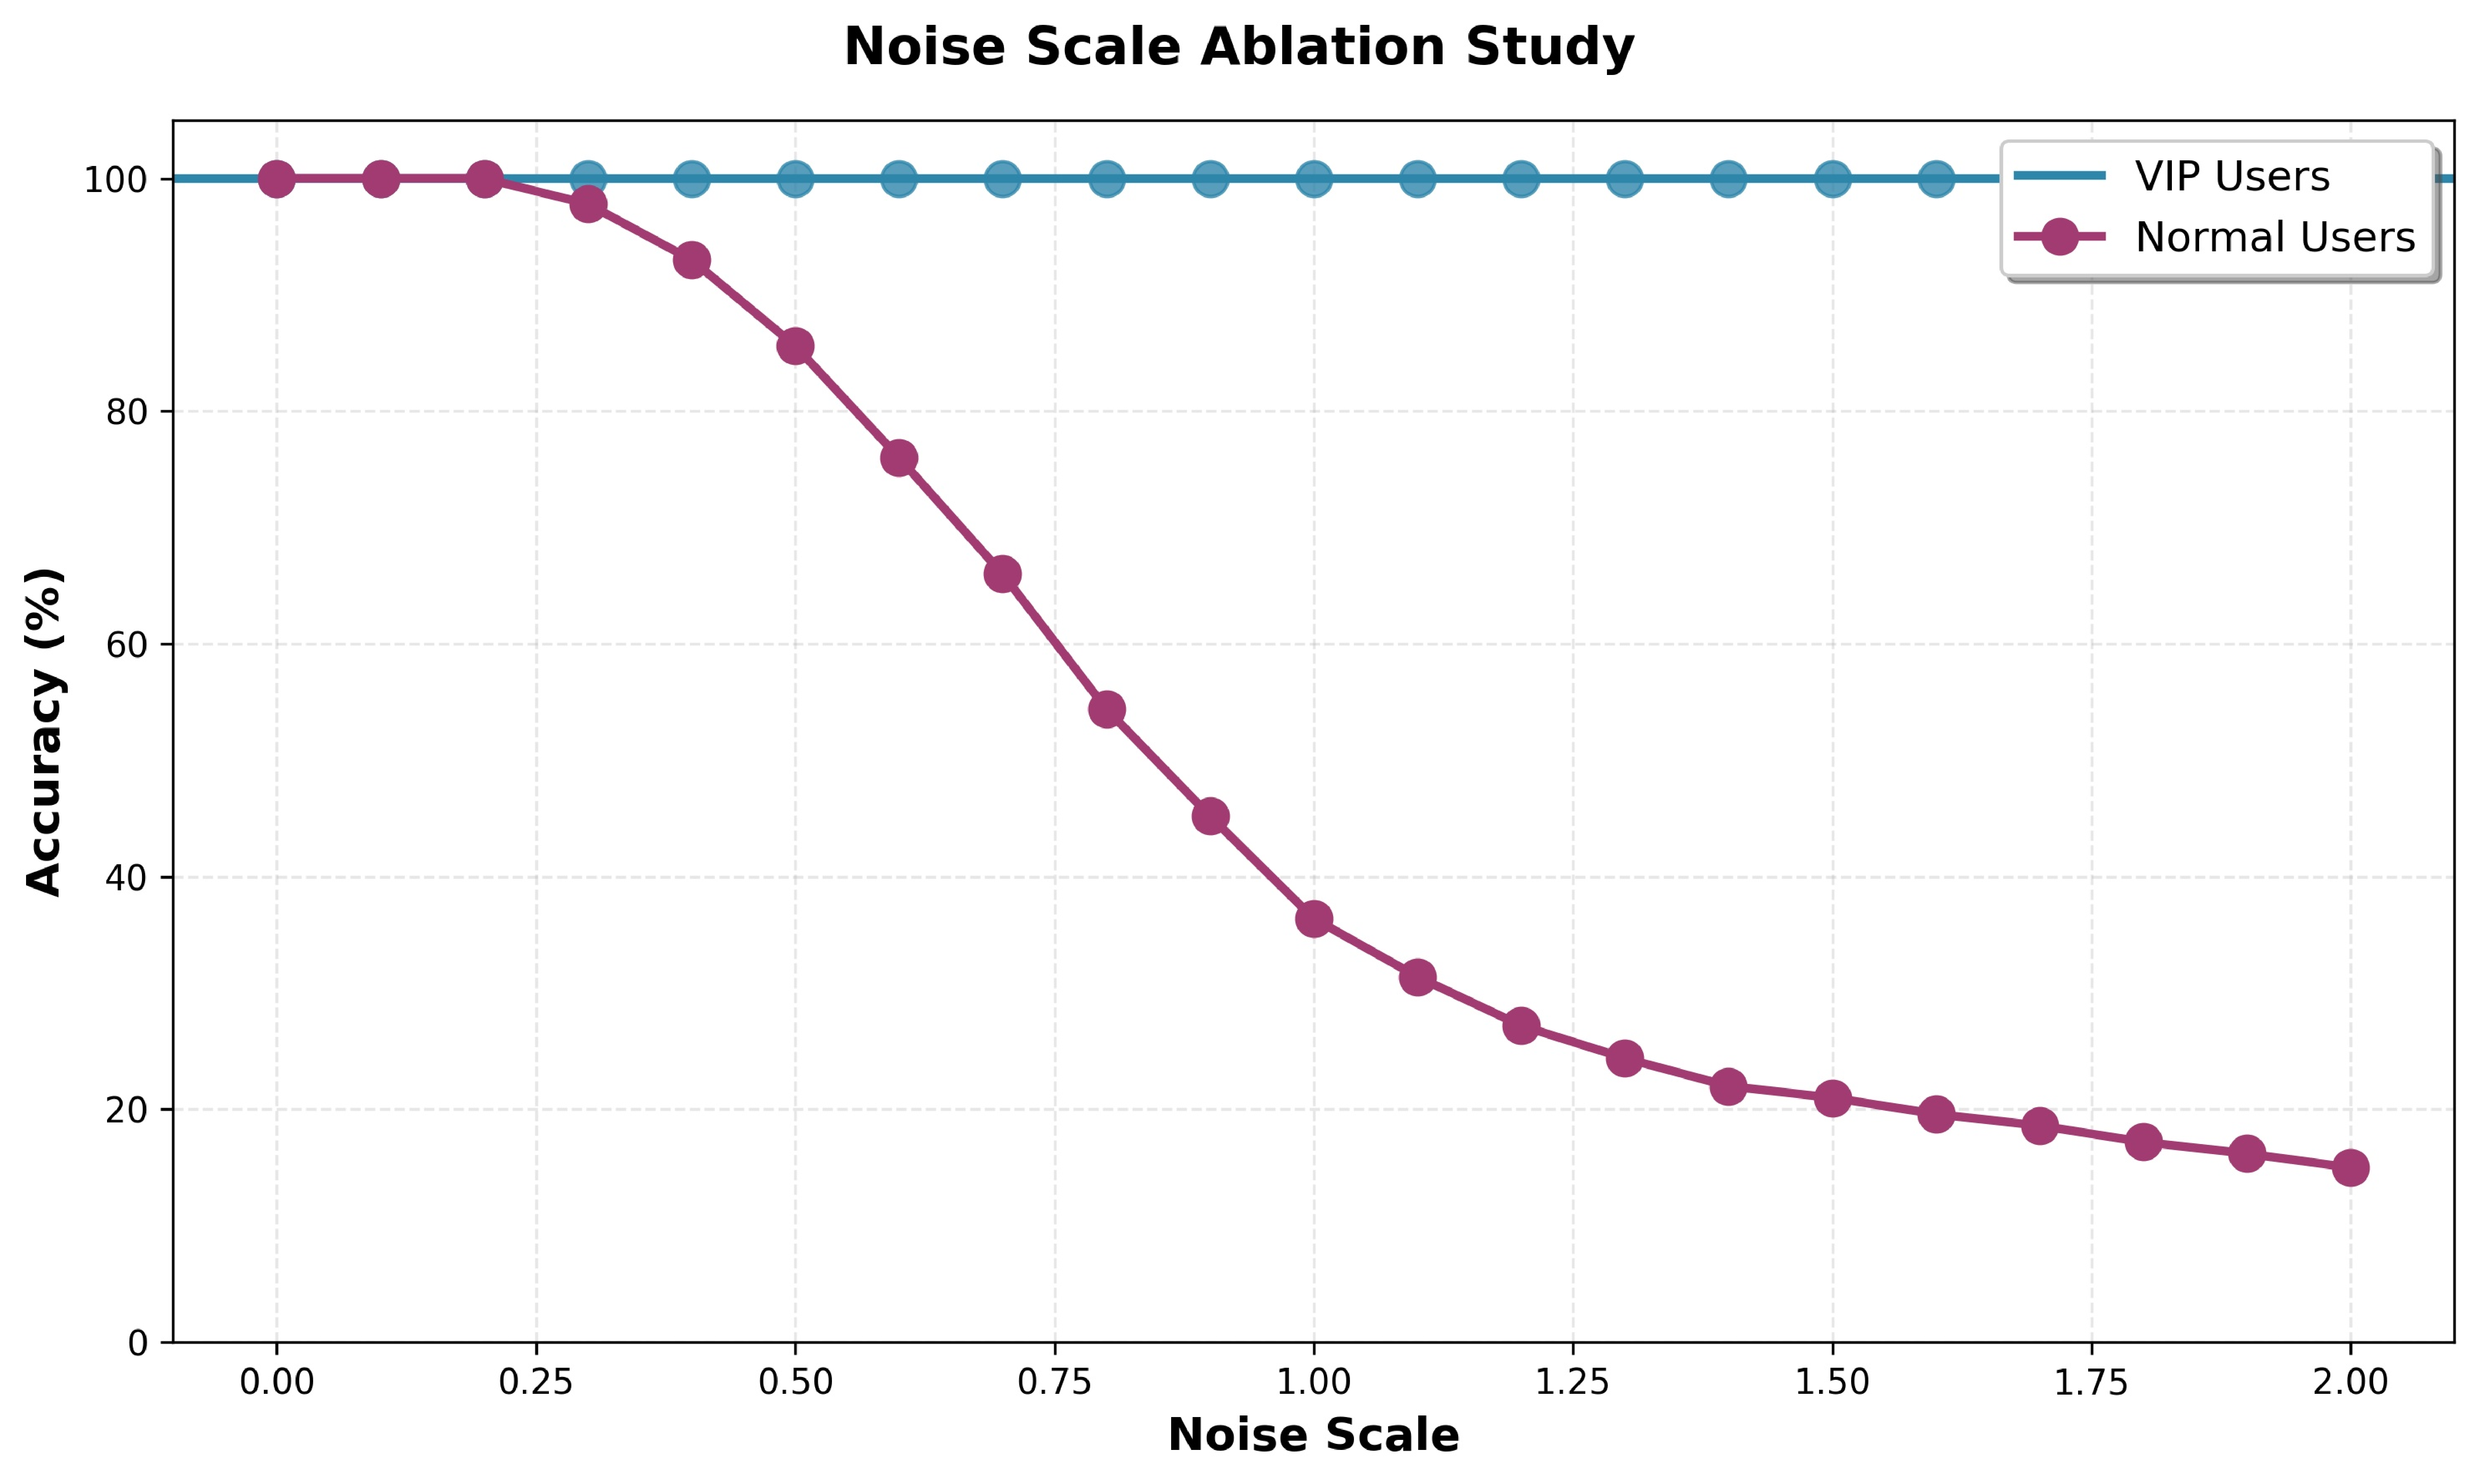
\includegraphics[width=\textwidth,height=0.66\textheight,keepaspectratio]{noise_scale_ablation.pdf}
    \vspace{0.1cm}
    \begin{center}\footnotesize
        VIP accuracy stays ${\approx}99.8\%$ across all $\lambda$; unauthorized accuracy declines smoothly --- granular control from subtle degradation to full lockout, no retraining.
    \end{center}
\end{frame}

\begin{frame}{Backup --- Channel Selector Ablation}
    \centering
    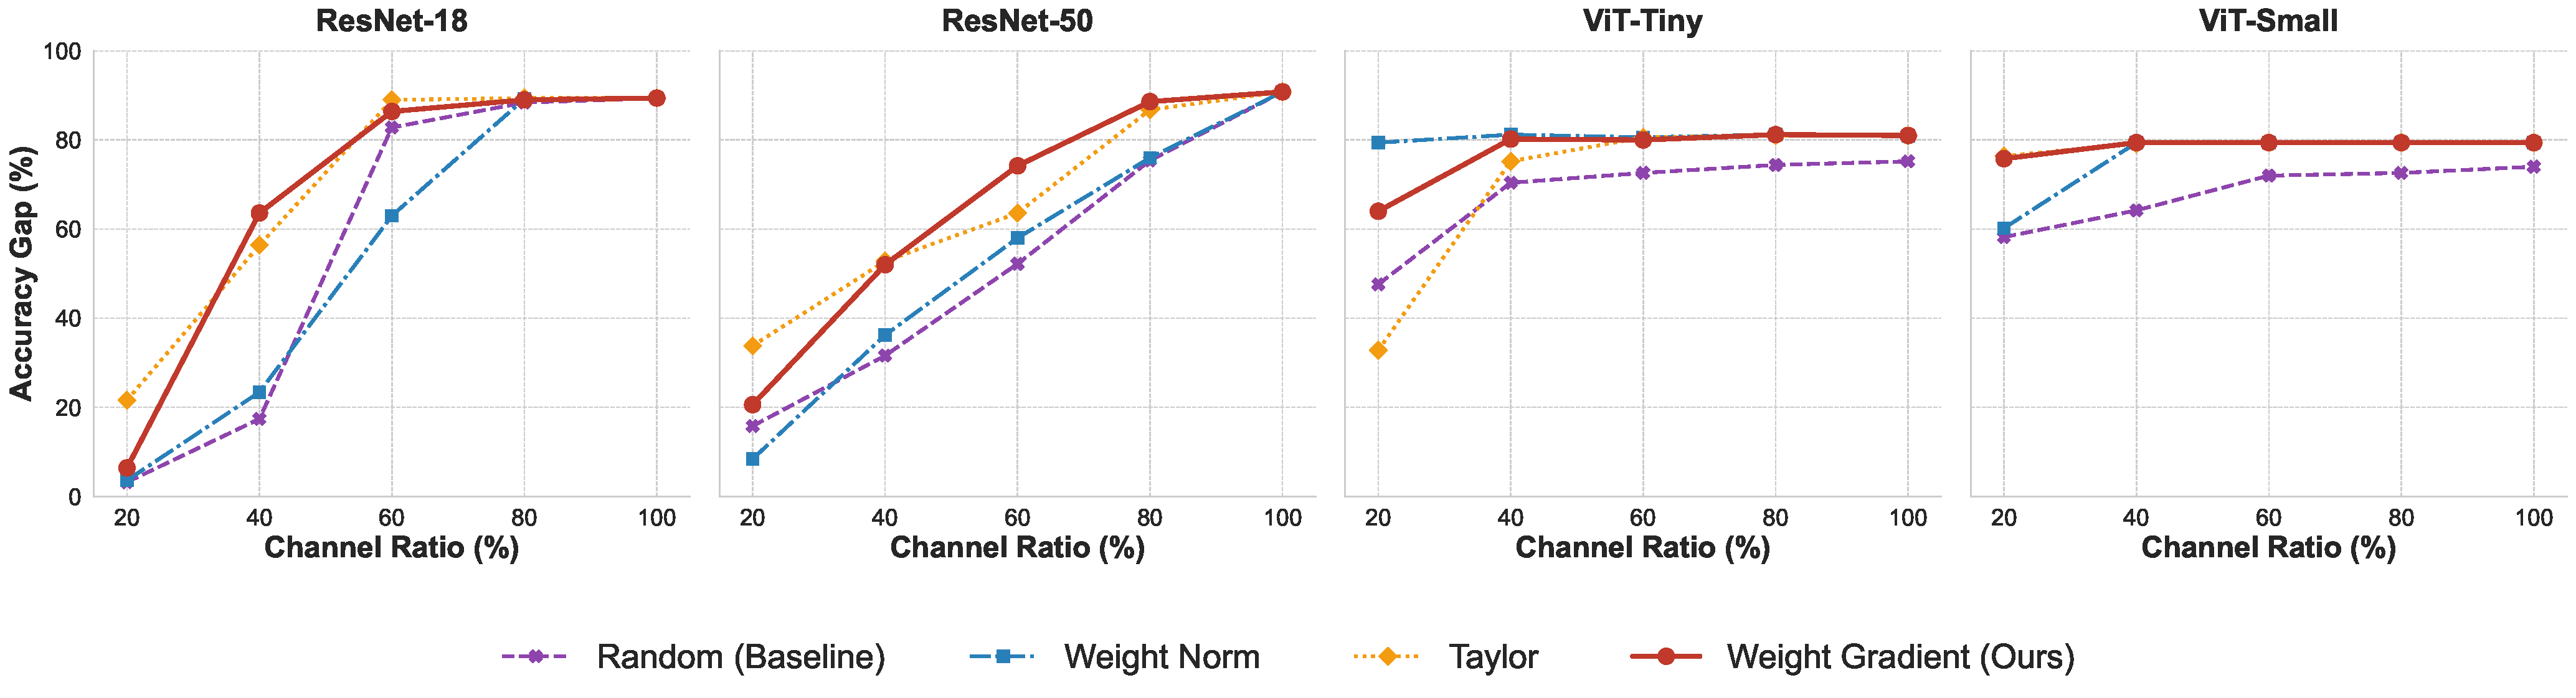
\includegraphics[width=\textwidth,height=0.62\textheight,keepaspectratio]{exp2_1x4.pdf}
    \vspace{0.1cm}
    \begin{center}\footnotesize
        Weight-Gradient selection beats Taylor, Weight-Norm, and Random; perturbing 40--60\% of channels matches full-channel neutralization (e.g.\ ResNet-50: 75\% vs 52\% gap for Taylor at 60\%).
    \end{center}
\end{frame}

\begin{frame}{Backup --- Fine-Tuning Robustness}
    \centering
    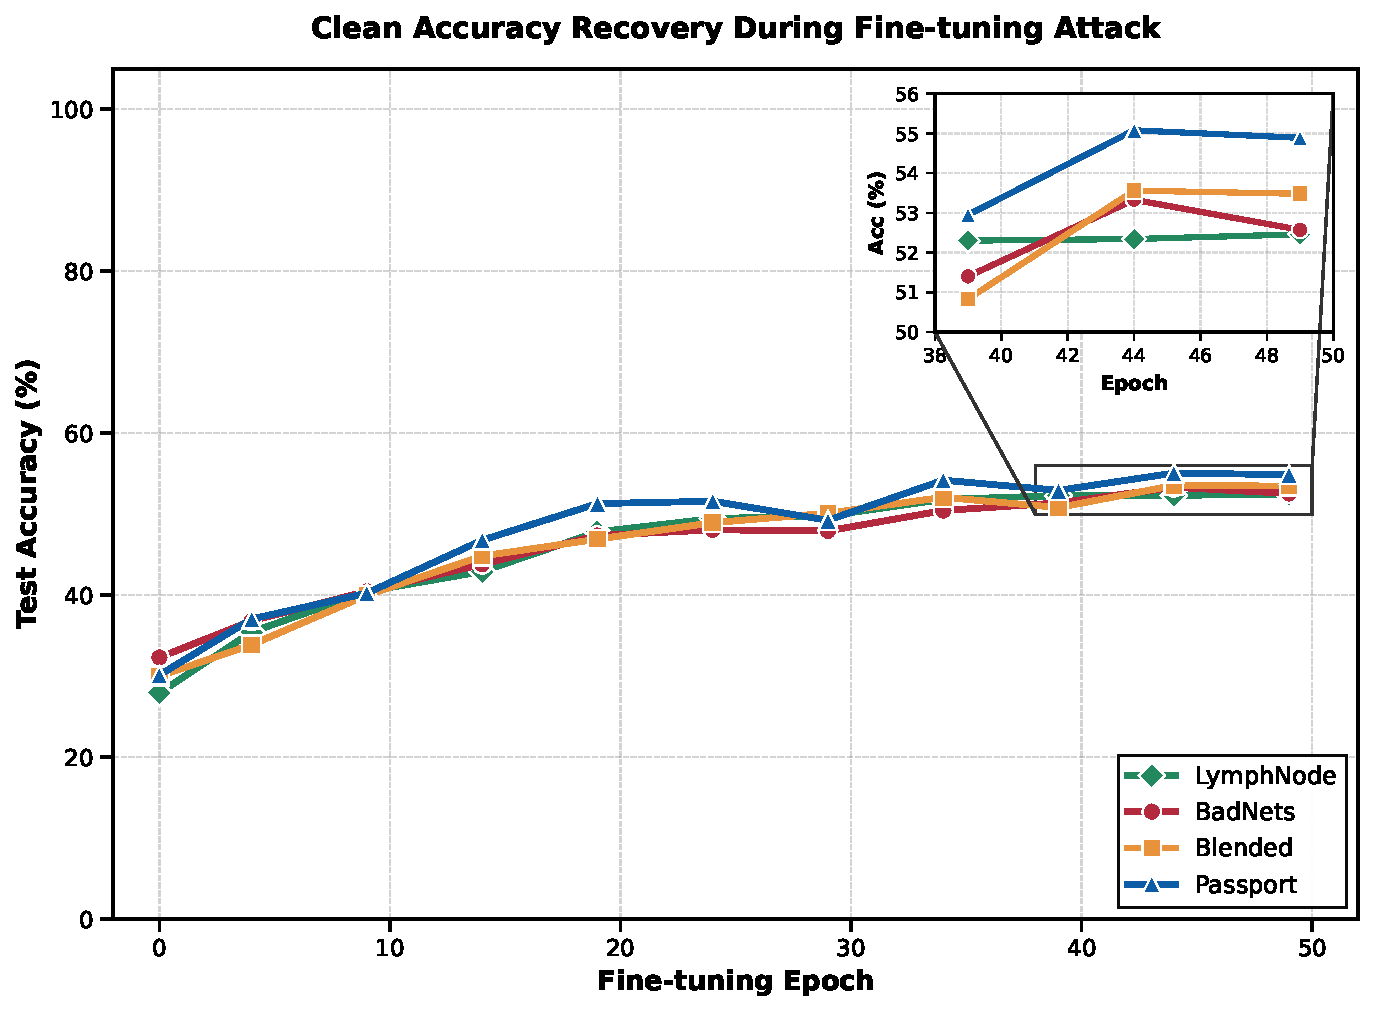
\includegraphics[width=\textwidth,height=0.64\textheight,keepaspectratio]{finetuning_attack.pdf}
    \vspace{0.1cm}
    \begin{center}\footnotesize
        50 epochs of SGD on 10\% clean data recover clean accuracy to only 52.5\% (orig.\ ${\approx}95\%$) --- comparable to structural Passport, far below usable fidelity.
    \end{center}
\end{frame}

\begin{frame}{Backup --- JPEG Compression Robustness}
    \small
    \begin{center}
    \setlength{\tabcolsep}{8pt}\renewcommand{\arraystretch}{1.25}
    \begin{tabular}{c|ccccc}
        \toprule
        \multirow{2}{*}{\textbf{Quality $Q$}} & \multicolumn{5}{c}{\textbf{Iterations $T$ (Authorization Success Rate)}} \\
        \cline{2-6}
         & 10 & 20 & 30 & 40 & 50 \\
        \midrule
        80 & 15.6\% & 82.4\% & 96.5\% & 99.1\% & 99.8\% \\
        70 & 2.3\%  & 45.8\% & 81.2\% & 93.7\% & 98.4\% \\
        60 & 0.0\%  & 8.5\%  & 35.2\% & 62.8\% & 85.6\% \\
        \bottomrule
    \end{tabular}
    \end{center}
    \vspace{0.3cm}
    \centering\footnotesize Iterative embedding hardens credentials against lossy channels: even aggressive Q60 reaches 85.6\% authorization success after 50 iterations.
\end{frame}

\end{document}
